\documentclass[12pt, a4paper]{article}

\usepackage[utf8]{inputenc}
% Limit the page margin to only 1 inch.
\usepackage[margin=1in]{geometry}

%Imports biblatex package
\usepackage[
backend=biber,
style=alphabetic
]{biblatex}
\addbibresource{../../algs4e.bib}

% Enables the `align' environment.
\usepackage{amsmath}
% Provides useful environments, such as:
% - \begin{proof} ...\end{proof}
\usepackage{amsthm}
\usepackage[most]{tcolorbox}

\newtheorem*{proposition}{Proposition}

% Enables using \mathbb{}, for example \mathbb{N} for the set of natural numbers.
\usepackage{amssymb}

% Allows using letters in enumerate list environment. Use, for example:
%\begin{enumerate}[label=(\alph*)]
% ...
%\end{enumerate}
\usepackage[inline]{enumitem}

% Enable importing external graphic files and provides useful commannds, like \graphicspath{}
\usepackage{graphicx}
% Images are located in a directory called images in the current directory.
\graphicspath{{./images/}}

% Make links look better by default.
% See: https://tex.stackexchange.com/questions/823/remove-ugly-borders-around-clickable-cross-references-and-hyperlinks
\usepackage[hidelinks]{hyperref}
\usepackage{xcolor}
\hypersetup{
	colorlinks,
	linkcolor={red!50!black},
	citecolor={blue!50!black},
	urlcolor={blue!80!black}
}


% Code Listings. Source:
% https://stackoverflow.com/questions/3175105/inserting-code-in-this-latex-document-with-indentation
\usepackage{listings}
\usepackage{color}

\definecolor{dkgreen}{rgb}{0,0.6,0}
\definecolor{gray}{rgb}{0.5,0.5,0.5}
\definecolor{mauve}{rgb}{0.58,0,0.82}

\lstset{frame=tb,
	language=Java,
	aboveskip=3mm,
	belowskip=3mm,
	showstringspaces=false,
	columns=flexible,
	basicstyle={\small\ttfamily},
	numbers=none,
	numberstyle=\tiny\color{gray},
	keywordstyle=\color{blue},
	commentstyle=\color{dkgreen},
	stringstyle=\color{mauve},
	breaklines=true,
	breakatwhitespace=true,
	tabsize=3
}

\newcommand{\prob}{\text{P}}
%\newcommand{\complement}{\mathsf{c}}

% Define an environment called "ex" (for Exercise) so that I can do: \begin{ex}{1.5}...\end{ex}
\newenvironment{ex}[2][Exercise]
{\par\medskip\noindent \textbf{#1 #2.}}
{\medskip}

% Define a solution environment, similar to ex (exercise) environment.
\newenvironment{sol}[1][Solution]
{\par\medskip\noindent \textbf{#1.} }
{\medskip}

\begin{document}
	\noindent Sergio E. Garcia Tapia \hfill
	
	\noindent \emph{Algorithms} by Sedgewick and Wayne (4th edition) \cite{sedgewick_wayne}\hfill
	
	\noindent January 09, 2025\hfill 
	\section*{4.1: Undirected Graphs}
	\begin{ex}{1}
		What is the maximum number of edges in a graph with $V$ vertices and no parallel
		edges? What is the minimum number of edges in a graph with $V$ vertices, none of
		which are isolated (have degree $0$)?
	\end{ex}
	\begin{sol}
		No parallel edges means that at most one edge connects any two given nodes.
		For any vertex $v_i$, there are $V$ possible edge candidates, including $v_0$
		itself (because loops are not disallowed, we can assume they are allowed).
		Then, for $v_1$, there are $V-1$ edges allowed: one for $v_1$, and one for each
		other vertex, except $v_0$. Continuing this way, we find that there is
		a maximum of $V!$ ($V$ factorial) edges.
		
		If $V$ is even, then the minimum is $V / 2$, since we can pair all vertices.
		If $V$ is odd, it is $\lfloor V / 2\rfloor + 1$.
	\end{sol}
	\begin{ex}{2}
		Draw, in the style of the figure in the text (page 524), the adjacency lists
		built by \texttt{Graph}'s input stream constructor for the file \texttt{tinyGex2.txt}
		depicted at left (input from \texttt{tinyGex2.txt}).
		\begin{lstlisting}[language={}]
12
16
 8  4
 2  3
 1 11
 0  6
 3  6
10  3
 7 11
 7  8
11  8
 2  0
 6  2
 5  2
 5 10
 5  0
 8  1
 4  1
		\end{lstlisting}
	\end{ex}
	\begin{sol}
		See Figure~\ref{fig:ex-02}.
		\begin{figure}
			\centering
			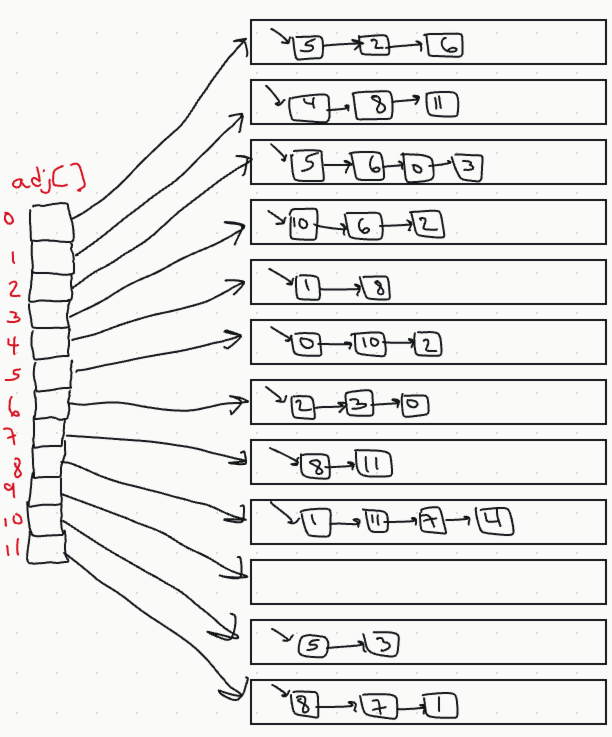
\includegraphics[width=0.5\textwidth]{exercise-02}
			\caption{Adjacency list representation for undirected graph from \texttt{tinyGex2.txt}}
			\label{fig:ex-02}
		\end{figure}
	\end{sol}
	\begin{ex}{3}
		Create a copy constructor for \texttt{Graph} that takes as input a graph
		\texttt{G} and creates and initializes a new copy of the graph. Any changes
		a client makes to \texttt{G} should not affect the newly created graph.
	\end{ex}
	\begin{sol}
		See \texttt{com.segarciat.algs4.ch4.sec1.ex03}.
	\end{sol}
	\begin{ex}{4}
		Add a method \texttt{hasEdge()} to \texttt{Graph} which takes two \texttt{int}
		arguments \texttt{v} and \texttt{w} and returns \texttt{true} if the graph has
		an edge \texttt{v-w}, \texttt{false} otherwise.
	\end{ex}
	\begin{sol}
		See \texttt{com.segarciat.algs4.ch4.sec1.ex04}.
	\end{sol}
	\begin{ex}{5}
		Modify \texttt{Graph} to disallow parallel edges and self-loops.
	\end{ex}
	\begin{sol}
		See \texttt{com.segarciat.algs4.ch4.sec1.ex05}.
	\end{sol}
	\begin{ex}{6}
		Consider the four-vertex graph with edges \texttt{0-1}, \texttt{1-2}, \texttt{2-3},
		and \texttt{3-0}. Draw an array of adjacency-lists that could \emph{not} have been
		built calling \texttt{addEdge()} for these edges \emph{no matter what order}.
	\end{ex}
	\begin{sol}
		\begin{figure}
			\centering
			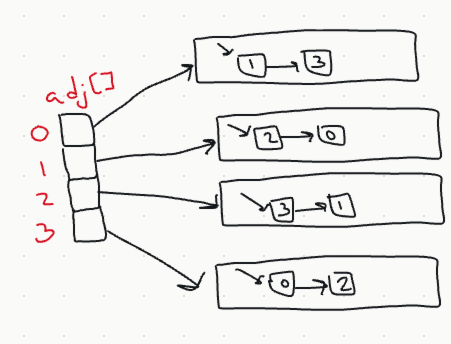
\includegraphics[width=0.3\textwidth]{exercise-06}
			\caption{Impossible adjacency-lists for a four-vertex graph with edges
			\texttt{0-1}, \texttt{1-2}, \texttt{2-3}, and \texttt{3-0}.}
			\label{fig:ex-06}
		\end{figure}
		See Figure~\ref{fig:ex-06}. The contents suggest that
		\begin{enumerate}
			\item According to 0's adjacency list, \texttt{0-3} comes before \texttt{0-1}.
			\item According to 3's adjacency list, \texttt{2-3} comes before \texttt{0-3}.
			\item According to 2's adjacency list, \texttt{1-2} comes before \texttt{2-3}.
			\item According to 1's adjacency list, \texttt{0-1} comes before \texttt{1-2}.
		\end{enumerate}
		According to the first three, the implied order is
		\begin{lstlisting}[language=java]
1-2
2-3
0-3
0-1
		\end{lstlisting}
		but then 1's adjacency list says that \texttt{0-1} comes before \texttt{1-2},
		which contradicts that \texttt{0-1} comes last in the list above. This can
		be seen from the adjacency lists because there must be first pair, which means
		that there is a pair of vertices \texttt{v} and \texttt{w} that are last in each
		other's adjacency lists. That would imply that \texttt{v-w} (or \texttt{w-v})
		was the first edge inserted. That doesn't happen in the figure, however.
	\end{sol}
	\begin{ex}{7}
		Develop a test client for \texttt{Graph} that reads a graph from the input stream
		named as command-line argument and then prints it, relying on \texttt{toString()}.
	\end{ex}
	\pagebreak
	\printbibliography
\end{document}